\subsection*{DDR Trend Lines}

Figure~\ref{fig:ddr-trends} extends the main-text DDR trajectory plot (Figure~\ref{fig:ddr-trajectory}) by showing per-feature depth trends with individual generator traces overlaid.
$R^2$ values are computed from ordinary least-squares regression on depth-level means (five points per generator, one per depth 0--4), not per-sample regression; the annotated Spearman $\rho$ provides the complementary per-sample monotonicity measure.

\begin{figure}[t]
\centering
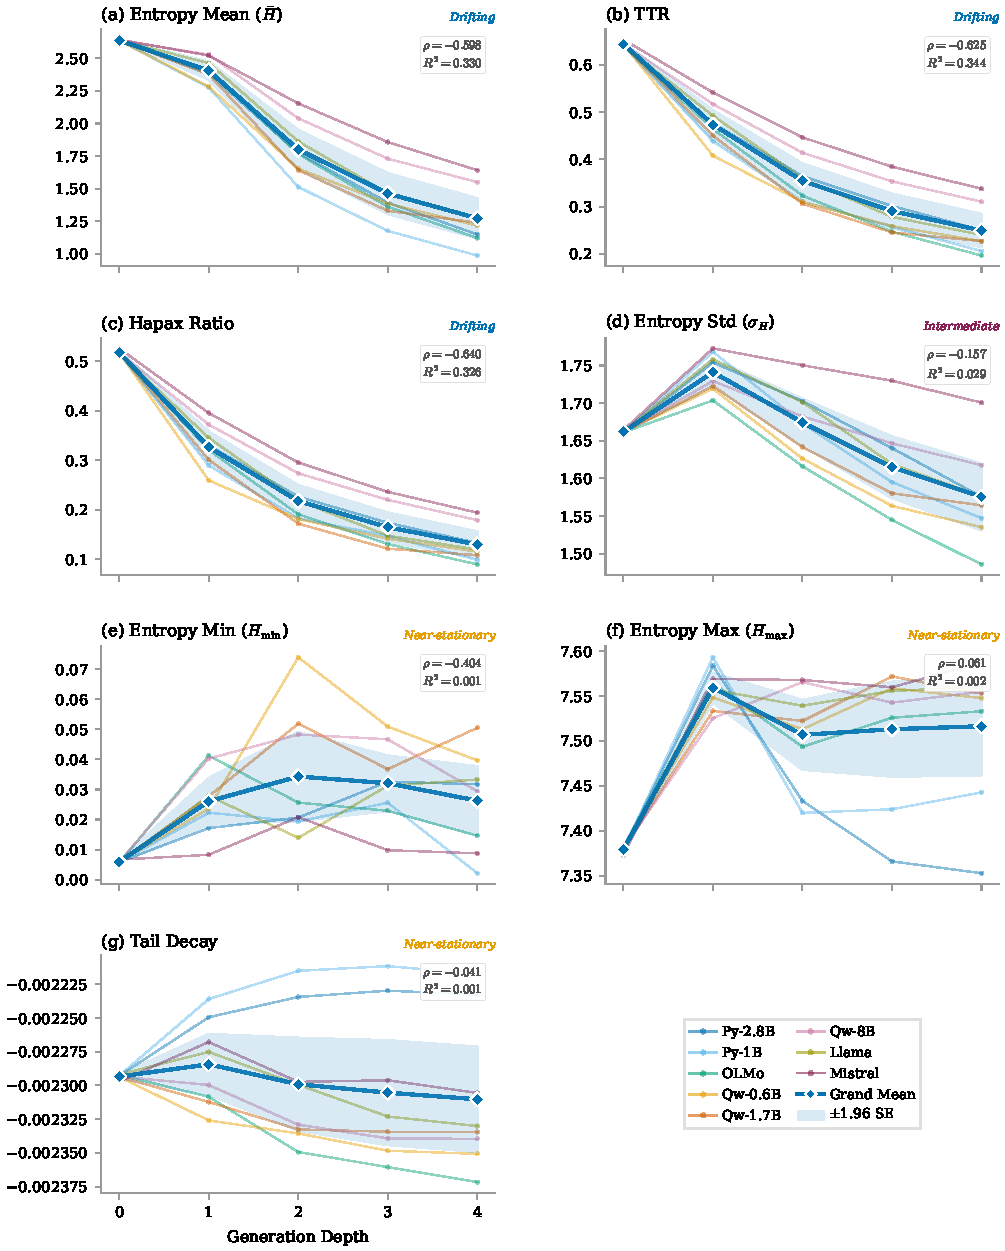
\includegraphics[width=\columnwidth]{fig_appendix_ddr_trends.pdf}
\caption{Per-feature depth trends. Bold line: pooled mean ($\pm$1.96\,SE shading) across all generators, colored by DDR zone (blue: drifting, wine: intermediate, amber: near-stationary). Thin traces: individual generators. Spearman $\rho$ and linear $R^2$ are annotated per panel.}
\label{fig:ddr-trends}
\end{figure}

\subsection*{UMAP Embedding}

Figure~\ref{fig:umap} shows a 2D UMAP projection of the 7-feature space (7{,}500 stratified samples, StandardScaler normalization, $k$\,=\,30 neighbors, min\_dist\,=\,0.3).
Panel~(a) reveals a depth gradient from gen-0 through gen-4, with progressive overlap at deeper generations consistent with the convergence that motivates the gen-2+ class collapse.
Panel~(b) shows the 3-class view: gen-0 forms a separable cluster, while gen-1 and gen-2+ overlap substantially, explaining the classification difficulty at this boundary.

\begin{figure}[t]
\centering
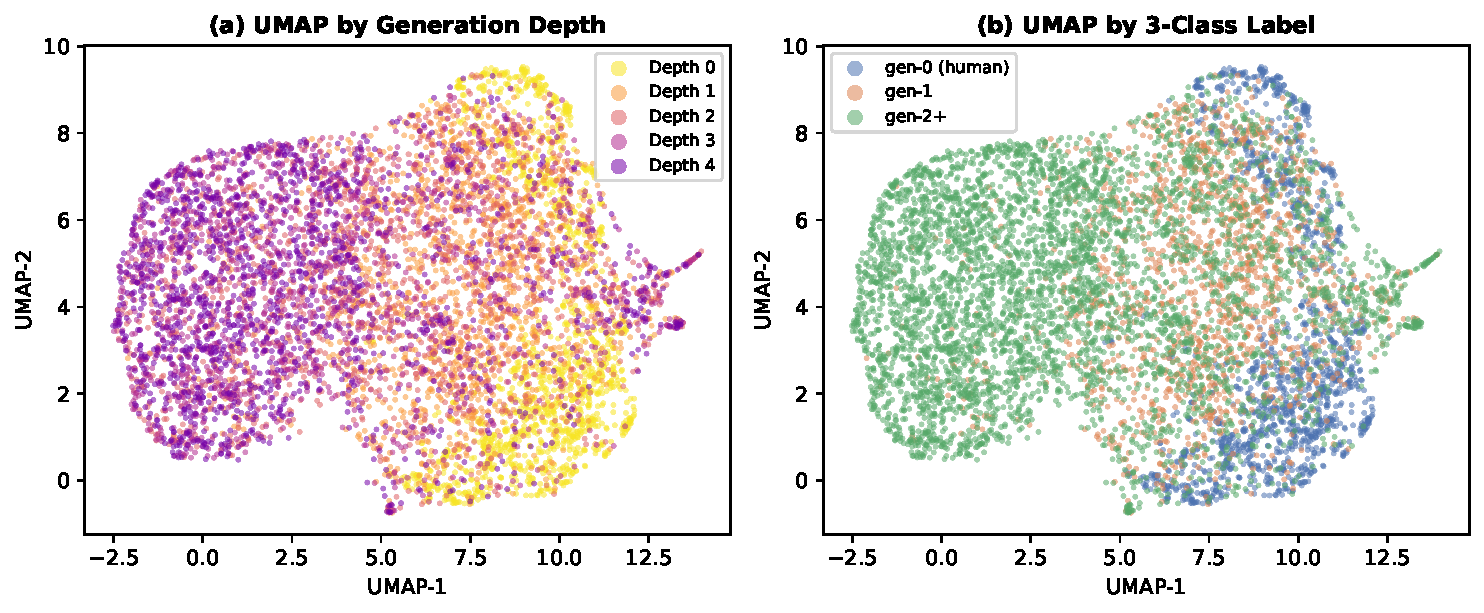
\includegraphics[width=\columnwidth, trim=0 0 356pt 0, clip]{fig_appendix_umap.pdf}\\[-2pt]
{\small (a) Colored by raw generation depth (0--4)}\\[6pt]
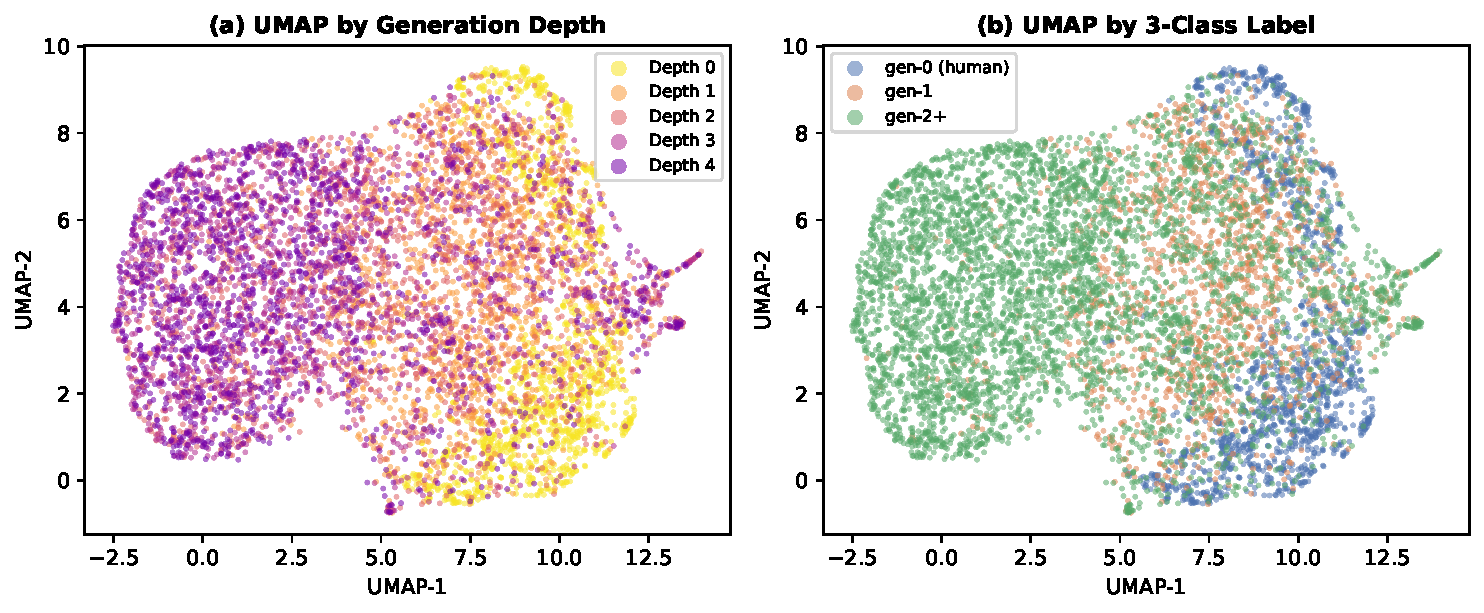
\includegraphics[width=\columnwidth, trim=356pt 0 0 0, clip]{fig_appendix_umap.pdf}\\[-2pt]
{\small (b) Colored by 3-class label}
\caption{UMAP 2D projection of the 7-feature space ($N$\,=\,7{,}500 stratified sample). (a) A gradient structure emerges, with deeper depths converging. (b) Gen-0 separates clearly; gen-1 and gen-2+ overlap, consistent with the high false-negative rate at the gen-1/gen-2+ boundary.}
\label{fig:umap}
\end{figure}
